\chapter[Cấu tạo và công dụng của kính lúp - Sự tạo ảnh của kính lúp]{Cấu tạo và công dụng của kính lúp \\ Sự tạo ảnh của kính lúp}
\section{Lý thuyết trọng tâm}
\subsection{Phân loại, công dụng và cấu tạo của kính lúp}
\subsubsection{Phân loại kính lúp}
Phân loại theo mục đích sử dụng
\begin{itemize}
	\item Kính lúp đọc sách: sử dụng để đọc sách báo $f$ nhỏ   . 
	\item Kính lúp sửa đồng hồ: được sử dụng trong sửa chữa đồng hồ, thường loại kính lúp này đeo mắt giúp người thợ rảnh tay trong quá trình sửa chữa. 
	\item Kính lúp sửa điện thoại, linh kiện điện tử: dùng để sửa chữa điện thoại, bảng mạch… thường sử dụng để bàn.
	\item Kính lúp soi kim cương: được sử dụng để soi vàng bạc đá quý, kim cương,...loại này thường rất nhỏ gọn và cầm tay. 
	\item Kính lúp soi vải: thường sử dụng để soi vải, cùng với thước chia để đếm mật độ vải sợi. 
\end{itemize}	

\subsubsection{Công dụng của kính lúp}

Kính lúp là dụng cụ quang bổ trợ cho mắt để quan sát các vật nhỏ.
\subsubsection{Cấu tạo của kính lúp}
\begin{center}
	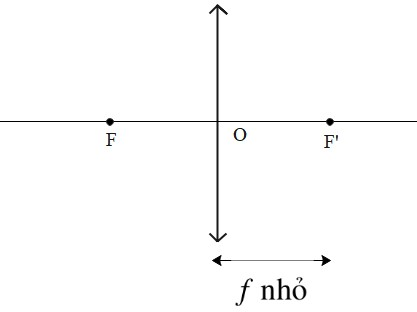
\includegraphics[scale=0.5]{../figs/VN11-PH-41-L-029-1-h42.jpg}
\end{center}

Kính lúp thực chất là \textit{thấu kính hội tụ}, hay hệ thấu kính ghép tương đương với một thấu kính hội tụ có tiêu cự nhỏ (cỡ vài cen-ti-mét).

Tính chất của kính lúp giống hoàn toàn thấu kính hội tụ. 

\subsection{Sự tạo ảnh bởi kính lúp}
Nguyên tắc bắt buộc khi sử dụng kính lúp là  
\begin{itemize}
	\item vật phải đặt cách thấu kính một khoảng \textit{nhỏ hơn tiêu cự.}
	\item ảnh phải có vị trí nằm ở trong khoảng nhìn rõ của mắt.
\end{itemize}

Ta cần điều chỉnh vị trí của vật hoặc kính, sao cho ảnh của vật hiện trong khoảng nhìn rõ của mắt hay chính là khoảng từ điểm cực viễn đến điểm cực cận của mắt. Cách quan sát và điều chỉnh như vậy gọi là cách ngắm chừng.

Ảnh mà ta thu được là ảnh ảo, cùng chiều, lớn hơn vật thể thật và không thể hứng được trên màn.
\begin{center}
	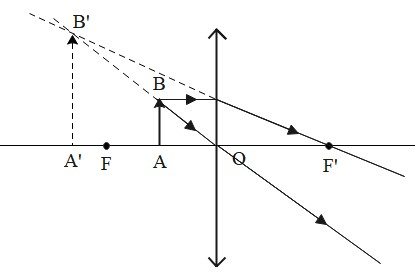
\includegraphics[scale=0.8]{../figs/VN11-PH-41-L-029-1-h43.jpg}
\end{center}

Góc trông vật là góc tạo bởi hai tia sáng xuất phát từ hai điểm A và B tới mắt.
\begin{center}
	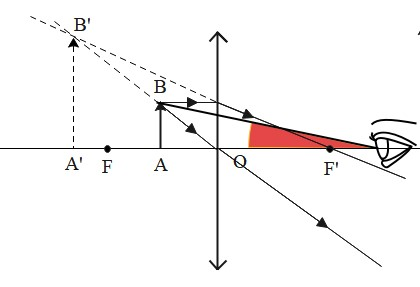
\includegraphics[scale=0.8]{../figs/VN11-PH-41-L-029-1-h44.jpg}
\end{center}


Góc trông ảnh chính là góc tạo bởi tia sáng xuất phát từ hai điểm A’ và B’ tới mắt. 
\begin{center}
	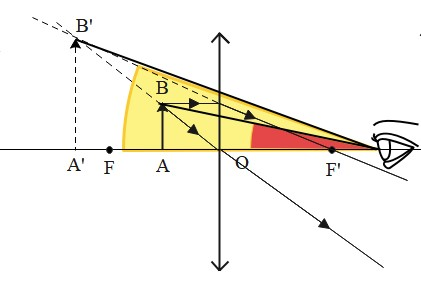
\includegraphics[scale=0.8]{../figs/VN11-PH-41-L-029-1-h45.jpg}
\end{center}

Góc này \textbf{nhỏ hơn nhiều} so với góc trông ảnh qua thấu kính.

Kính lúp giúp ta tạo ra ảnh dưới \textbf{góc trông ảnh lớn hơn góc trông vật} khi ta nhìn trực tiếp bằng mắt thường.

Với cùng một vật và vị trí vật đến thấu kính là không đổi, kính lúp có tiêu cự khác nhau sẽ tạo ra ảnh ảo to, nhỏ khác nhau,  góc trông ảnh qua thấu kính cũng to, nhỏ khác nhau. 

Tiêu cự càng nhỏ thì tạo ra ảnh càng lớn hay góc trông ảnh càng lớn và ngược lại.


\section{Bài tập}
\begin{dang}{Cấu tạo, công dụng của kính lúp \\và sự tạo ảnh bởi kính lúp}
\end{dang}

\viduii{1}{
Phát biểu nào sau đây về kính lúp là \textbf{không đúng}?
\begin{mcq}
	\item Kính lúp là dụng cụ quang học bổ trợ cho mắt làm tăng góc trông để quan sát một vật nhỏ.
	\item Vật cần quan sát đặt trước kính lúp cho ảnh thật lớn hơn vật.
	\item Kính lúp đơn giản là một thấu kính hội tụ có tiêu cự ngắn.
	\item Kính lúp có tác dụng làm tăng góc trông ảnh bằng cách tạo ra một ảnh ảo lớn hơn vật và nằm trong giới hạn nhìn rõ của mắt.
\end{mcq}}{
\begin{center}
	\textbf{Hướng dẫn giải:}
\end{center}

{ Vật cần quan sát đặt trước kính lúp cho ảnh ảo lớn hơn vật chứ không phải cho ảnh thật. 
	
\textbf{	Đáp án: B.}
}'
}
\viduii{1}{
Phát biểu nào sau đây về kính lúp là \textbf{không đúng}?
\begin{mcq}
	\item Khi quan sát một vật nhỏ qua kính lúp ta phải điều chỉnh khoảng cách giữa vật và kính để ảnh của vật nằm trong khoảng nhìn rõ của mắt.
	\item Khi quan sát một vật nhỏ qua kính lúp ta phải đặt vật trong khoảng tiêu cự của kính sao cho ảnh của vật nằm trong khoảng nhìn rõ của mắt.
	\item Khi quan sát một vật nhỏ qua kính lúp ta phải đặt vật ngoài khoảng tiêu cự của kính sao cho ảnh của vật nằm trong khoảng nhìn rõ của mắt.
	\item Khi quan sát một vật nhỏ qua kính lúp ta phải điều chỉnh ảnh của vật nằm ở điểm cực viễn của mắt để việc quan sát đỡ bị mỏi mắt.
\end{mcq}}{
\begin{center}
	\textbf{Hướng dẫn giải:}
\end{center}

{ Khi quan sát một vật nhỏ qua kính lúp ta phải đặt vật \textbf{trong} khoảng tiêu cự của kính sao cho ảnh của vật nằm trong khoảng nhìn rõ của mắt.
	
\textbf{	Đáp án: C.}
}



}